\documentclass[12pt]{article}

\usepackage{sbc-template}
\usepackage{placeins}
\usepackage{graphicx,url}
\usepackage{float}
\usepackage[brazil]{babel}   
%\usepackage[latin1]{inputenc}  
\usepackage[utf8]{inputenc}  
% UTF-8 encoding is recommended by ShareLaTex

     
\sloppy

\title{Primeiro Projeto de comunicações Móveis}

\author{Vítor Gabriel Lemos Lopes }

\address{Departamento de Engenharia de Comunicações \\ Universidade Federal do Rio Grande do Norte(UFRN)}


\begin{document} 
\maketitle


\begin{resumo} 
 No presente documento, foi feito um estudo da comunicação sem fio em um determinado ambiente controlado para saber como se comporta a potência do sinal, para isso foi simulado com a linguagem de programação \textit{Python}, de 7 estações rádio base(ERB) dispostas em uma determinada área para saber como se comporta usando\textit{ Okumura-Hata} e com um determinado sombramento.
\end{resumo}


\section{Introdução}
Na comunicação sem fio um sinal transmitido sofre basicamente 3 tipos de atenuação \textit{Primeiro}:\textit{Path Loss}, ou em português, perda de de percurso, que é a perda em função da distância percorrida pelo sinal, essa perda de potência é chamada de desvanecimento em larga escala. \textit{Segundo}: o Sombreamento, ou em inglês,\textit{Shadowing}, que também é um desvanecimento em larga escala que é uma perda de potência devido aos obstáculos encontrados no caminho do sinal, que refletem nesses determinados obstáculos, sejam prédios, construções ou relevo.\textit{Terceiro}: Os efeitos do multi-percurso e o doppler, que são os desvanecimento em pequena escala, ou também conhecido do inglês, \textit{Fading}, mas não iremos usar esse tipo de perda nesse trabalho.
\\
Para estudar os fenômenos dos desvanecimentos de larga escala, que é o que vamos abordar nesse trabalho, definimos a perda de percurso de acordo com o modelo de \textit{Okumura-Hata} COST231 que é encontrado no livro\textit{ RAPPAPORT, T.S.\textbf{ Comunicações sem fio},2 ed. Prentice-hall,2009, P. 99-100} que tem a seguinte formula:
\begin{eqnarray}
LHata=46.3 +33.9log_{10}(f) - 13.82log_{10}(ht) - a(hr,f)+ (44.9 - 6.55log_{10}(ht))log_{10}(d) + C
\end{eqnarray}
Onde
\begin{itemize}
    \item \textbf{Lhata}: a média da perda de percurso. Unidade: decibel(dB).
    \item \textbf{f}: frequência de transmissão. Unidade megahertz(MHz).
    \item \textbf{ht}: altura efetiva da antena transmissora. Unidade: metro(m).
    \item \textbf{hr}:  altura efetiva da antena receptora. Unidade: metro(m).
    \item \textbf{d}:distância entre antena transmissora e receptora.Unidade: quilômetros (km).
    
\end{itemize}
O qual a(hr,f) para centros urbanos e f$\geq$ 300Mhz.
\begin{eqnarray}
a(hr,f)=3.2(log_{10}(11.75hr))^{2} -4.97
\end{eqnarray}
E a constante de offset para centros metropolitanos C= 3dB



\section{Experimento 1} \label{sec:firstpage}
O Primeiro experimento consiste em montar um grid em alguma linguagem de programação, e colocar 7 ERBs distanciadas simetricamente em formato de hexágono com a distância entre os pontos de medição de 50 metros (resolução espacial de 50m). \\
Nas figuras a seguir, feitas com código em Python, mostra a distribuição das 7 antenas nos centros dos hexágonos, lugares estes onde está situado os pontos de medição com maior potência.\\
Foi pedido como primeiro gráfico, ter como parâmetros um do raio do hexágono de 500M, e para efeito de calculo da perda de percurso pela formula COST231, uma transmissão de 20 Watts, frequência de 800 MHz, altura da antena transmissora de 32 m e altura da antena receptora de 1.5m.
\begin{figure}[!h]
\centering
    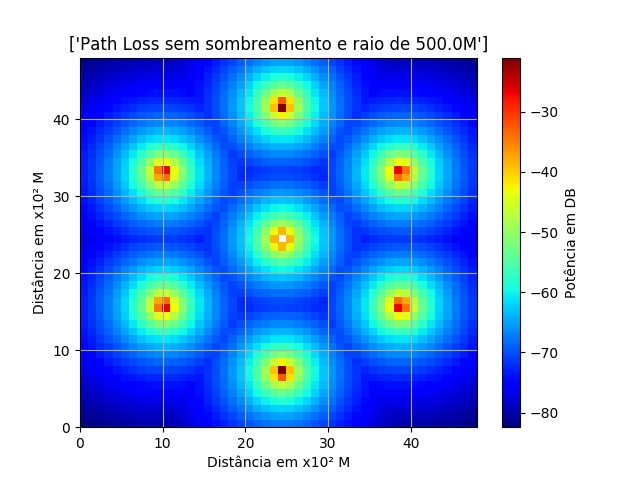
\includegraphics{800Mhzsvg.jpeg}
    \caption{800MHz}
\end{figure}
\FloatBarrier
Na figura 1 é possível perceber a localização das antenas transmissoras pelos pontos mais avermelhados, e a área de cobertura que elas estão mais fortes, isso é dado que as potências mostradas na figura estão em dB.\\
Na próxima figura, figura 2, são os mesmos parâmetros da figura 1 a diferença que foi mostrado a uma frequência de 1900 MHz.
\begin{figure}[h!]
    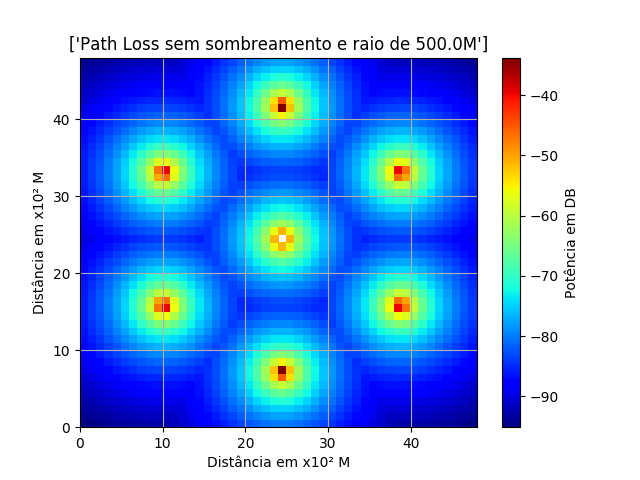
\includegraphics{1900Mhz.png}
    \caption{1900MHz}
\end{figure}
\FloatBarrier
Na figura 2, percebemos na semelhança na figura 1 e vemos que se comportam igual, diferenciando apenas na potência recebida por causa da frequência de transmissão.\\
Na próxima figura, figura 3, temos a mesma frequência de transmissão só que adicionamos o sombreamento que foi feito com a seguinte formula:
\begin{equation}
    Ltotal=LHata+X{_{\sigma }}
\end{equation}
Os quais LHata, foi o que foi calculado anteriormente e $X{_{\sigma }}$ e foi calculado como:
\begin{equation}
    X{_{\sigma }}= \sigma * randn(len(ERB),len(ERB[0))
\end{equation}
O $\sigma$ foi dado no projeto, que é de 8dB. o randn é uma função que foi utilizado da biblioteca numpy do Python que retorna uma distribuição normal aleatória, foi usando o tamanho da matriz das ERBs como argumento que é para ele retornar a mesma quantidade de pontos.
\begin{figure}[h!]
    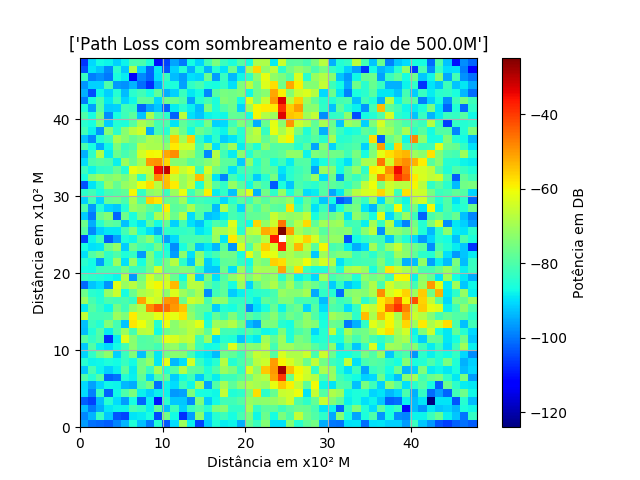
\includegraphics{shadow.png}
    \caption{1900MHz com sombreamento}
\end{figure}
\FloatBarrier
Com a posse da Figura 3 podemos fazer a comparação entre a figura 2 e a figura 3, as duas figuras tem a mesma frequência só que a figura 3 tem uma maior atenuação e de maneira aleatória em determinados pontos tem uma maior ou menor atenuação. Agora não mais tão semelhante quanto o da figura 1 e figura 2 que formavam imagens com hexágonos, agora na figura 3 não existe mais, assim podemos observar o efeito do sombreamento que é aleatório.

\section{Experimento 2}
Para o segundo experimento é pedido para verificar os pontos que tem uma potência menor do que -90 dBm, e descobrir qual é a potência de transmissão a qual no máximo 2\% dos pontos estejam abaixo de -90 dBm para as frequências de 800,1800,1900,2100 MHz todos com raio de 500 m, altura da antena transmissora de 32 m e da receptora 1.5 m, usando apenas a perda de percurso o COST231. Com posse desses dados, foi pedido também que para que fosse gerado um gráfico de barras com os resultados, o qual vemos a seguir:
\begin{figure}[h!]
    \centering
    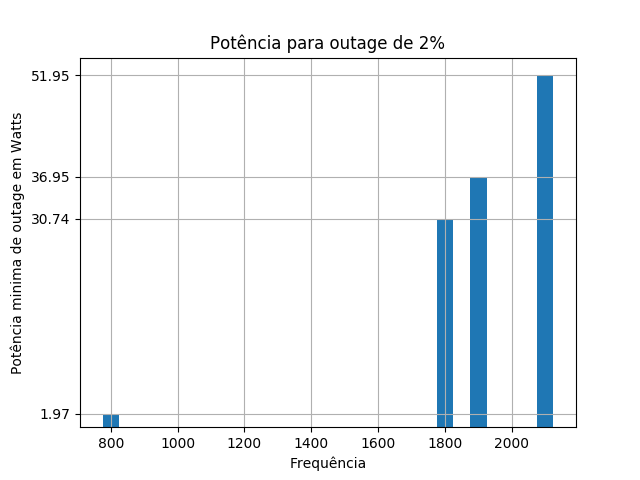
\includegraphics{potenciadeoutage.png}
    \caption{Potência de Outage}
    \label{fig:my_label}
\end{figure}
\FloatBarrier
Para descobrir a potência de Outage, foi feito uma função recursiva em Python, que tinha como retorno a potência em Watts a qual tinha como parada quando a função chegasse a uma porcentagem de transmissões abaixo de -90 dB ficasse entre 1.85 a 2\%. Com isso foram descobertos essas potências mostradas na figura 4 para cada frequência dada no problema.
É possível notar que esse gráfico cresce de forma logarítmica por causa que é transformado de watts para dBm para poder calcular a perda de percurso, e percebemos como a perda de percurso é severa em frequências mais altas.
\section{Conclusão}
Dado exposto no trabalho,o qual foram adquiridos conhecimentos sobre propagação e como se comporta o canal sem fio canal sem fio, que foi mostrado através de simulação. E este conhecimento e simulação foram a finalidade do projeto, fazendo o aluno ficar mais próximo de casos reais, que são as áreas de cobertura de cada estação rádio base e como está a potência em cada ponto do mapa, para poder escolher uma potência de transmissão correta e onde são as áreas de \textit{Handover} de acordo com nosso parâmetro de medição, e isso faz que seja crucial para o conhecimento de um engenheiro de telecomunicações.
\section{References}

\textit{ RAPPAPORT, T.S.\textbf{ Comunicações sem fio},2 ed. Prentice-hall,2009}
\end{document}